% NEWADDITION: Created methodology chapter to match ClassiFish structure
% This chapter describes the research methodology and system development approach

\chapter{Methodology}
\label{chap:methodology}

% NEWADDITION: Section structure based on ClassiFish reference and research best practices
\section{Research Methodology}
% This section will describe:
% - Research approach (applied research/development)
% - Mixed methods approach (technical development + user testing)
% - Research questions and objectives

{\color{maroon}
\section{System Architecture Design}
\label{sec:system_architecture_design}

The Consol system architecture integrates semantic similarity evaluation with user-centered interface design to create an effective recall assessment platform. Following established patterns in educational technology development, the architecture emphasizes modularity, scalability, and pedagogical effectiveness while ensuring seamless integration between natural language processing capabilities and user interaction requirements.

% Full page detailed tech stack architecture diagram
\begin{figure}[p]
\centering
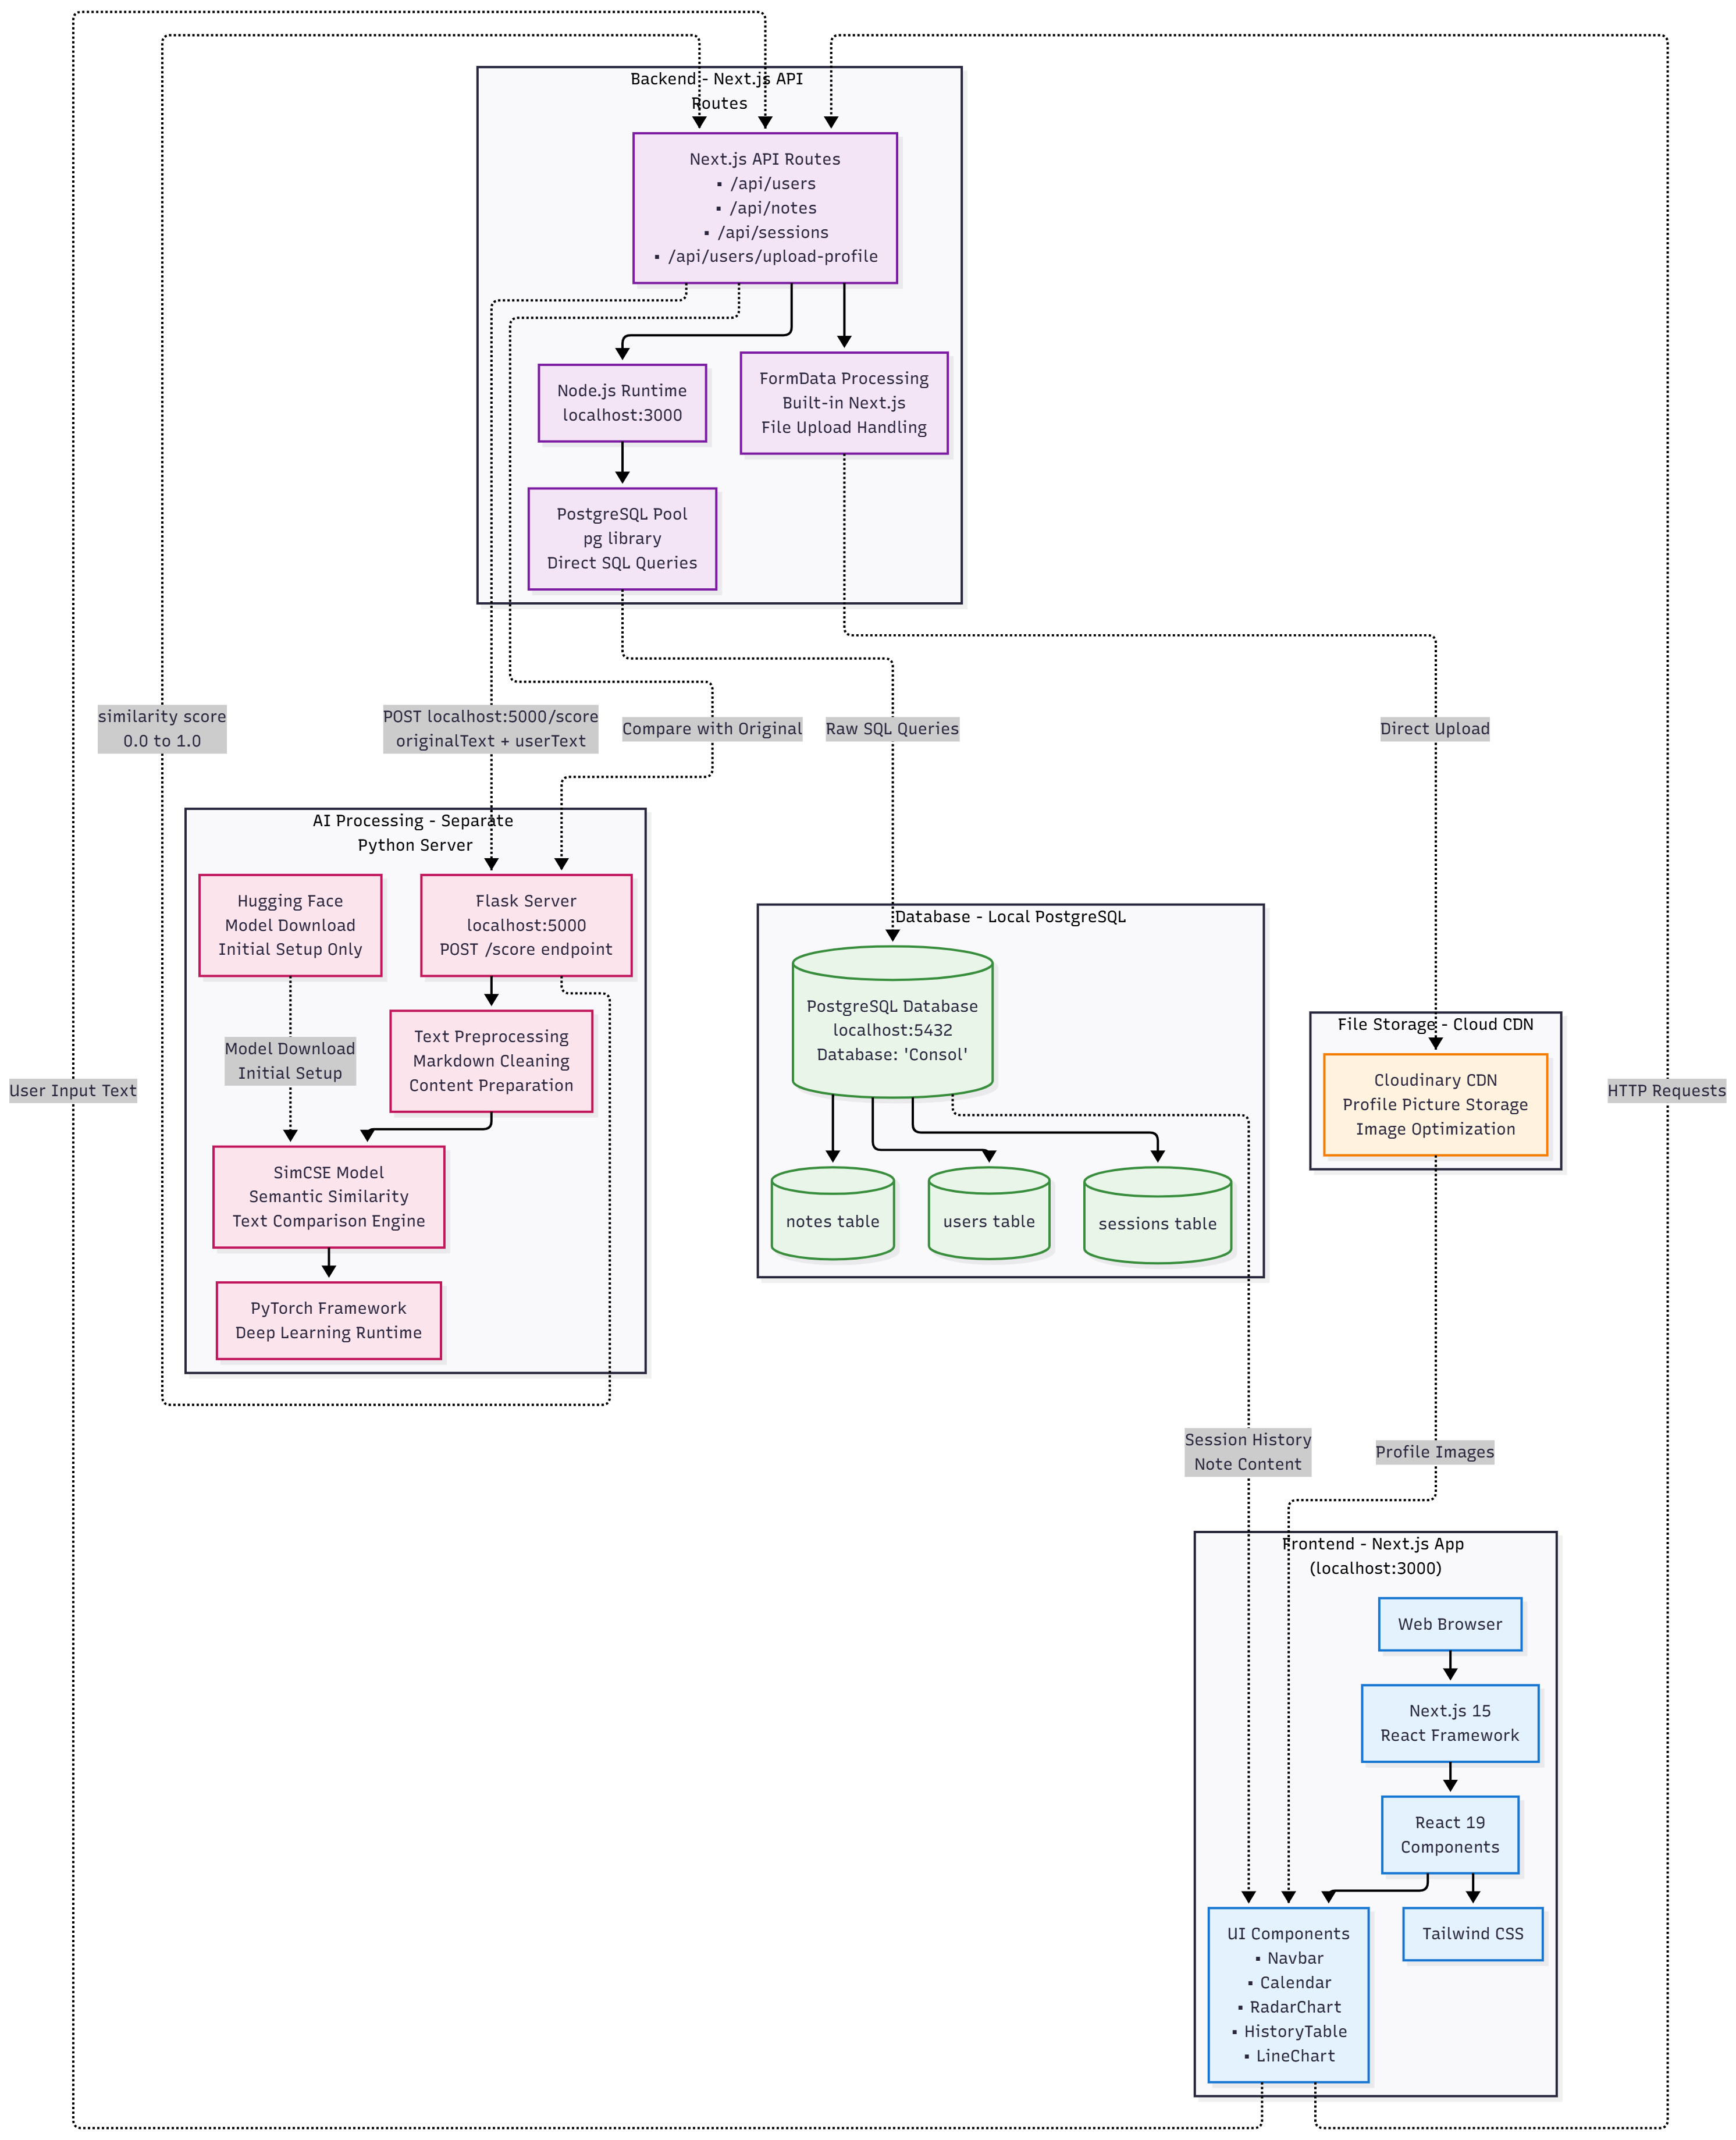
\includegraphics[width=0.95\textwidth]{images/tech_stack_architecture.png}
\caption[Detailed Technology Stack Architecture]{Comprehensive technology stack architecture diagram showing the complete integration from frontend React components through API layers to database and AI processing services. The architecture details specific technologies: Next.js 15 frontend with React 19 components, Node.js API layer with PostgreSQL database, Python Flask server for SimCSE processing, and external integrations for file storage and analytics. Each layer shows specific components, data flow patterns, and integration protocols essential for educational platform scalability and reliability.}
\label{fig:tech_stack_architecture}
\end{figure}

\subsection{Detailed Technology Stack Integration}

Beyond the core system architecture, the detailed technology stack provides granular insight into component interactions and data flow patterns essential for educational platform deployment. Figure \ref{fig:tech_stack_architecture} presents the comprehensive technology integration, highlighting specific frameworks, libraries, and services that enable Consol's educational effectiveness.

The multi-layered architecture ensures educational platform requirements including data security, user privacy, scalable assessment processing, and institutional integration capabilities. Each technology choice directly supports pedagogical objectives while maintaining technical excellence throughout the system.

\subsection{Architectural Overview}

The system architecture follows a client-server model where the frontend handles user interactions and immediate feedback presentation, while the backend manages semantic similarity computation, data persistence, and learning analytics. This separation enables independent scaling of user interface responsiveness and computational processing, crucial for educational applications that must maintain low-latency feedback while performing complex NLP operations.

The architectural design prioritizes educational outcomes over technical complexity, ensuring that technology choices directly support learning objectives rather than introducing unnecessary overhead. Each component serves specific pedagogical functions while maintaining technical coherence throughout the system.

\subsection{Technology Stack Selection}

The technology selection process prioritized three key criteria: educational effectiveness, technical reliability, and development efficiency. Each technology choice was evaluated based on its ability to support the core research objectives of semantic similarity assessment and user engagement optimization.

Frontend Architecture - Next.js was selected as the primary frontend framework due to its hybrid rendering capabilities that enable both static content delivery for consistent educational resources and server-side rendering for dynamic user interactions. The framework's automatic code splitting ensures optimal performance across diverse devices commonly used in educational settings, while its built-in optimization features reduce cognitive load through faster interface responsiveness.

React's component-based architecture facilitates the development of reusable educational interface elements, enabling consistent user experience across different assessment contexts. The virtual DOM implementation provides efficient updates to progress indicators and similarity feedback displays, essential for maintaining engagement during recall sessions.

Backend Architecture - The backend employs a Node.js runtime environment to maintain JavaScript consistency across the technology stack, reducing development complexity and enabling shared utility functions between frontend and backend components. This consistency supports rapid iteration and debugging, critical factors in educational software development where user experience requires frequent refinement.

PostgreSQL serves as the primary database system, chosen for its robust ACID compliance essential for maintaining accurate learning progress records and its support for complex queries required for learning analytics. The database's reliability ensures that student performance data remains consistent and recoverable, addressing institutional requirements for educational data integrity.

Semantic Processing Pipeline - The SimCSE implementation utilizes BERT-base-uncased as the foundational encoder, selected for its demonstrated performance in sentence similarity tasks and its compatibility with educational content processing. The encoder integration occurs through RESTful API endpoints that enable asynchronous processing, preventing similarity computation from blocking user interface responsiveness.

\textbf{Mathematical Foundation}: SimCSE implements unsupervised contrastive learning through the following loss function:
\begin{equation}
\ell_i = -\log \frac{e^{\text{sim}(h_i, h_i^+)/\tau}}{\sum_{j=1}^{N} e^{\text{sim}(h_i, h_j^+)/\tau}}
\end{equation}
where $h_i$ represents the hidden representation of input sentence $i$, $h_i^+$ denotes the positive sample (same sentence with different dropout), $\text{sim}(\cdot,\cdot)$ computes cosine similarity, $\tau$ is the temperature parameter controlling distribution sharpness, and $N$ represents the batch size.

The 768-dimensional embedding space exhibits structured semantic organization with dimensions 1-100 capturing basic semantic concepts, dimensions 101-300 encoding grammatical features, dimensions 301-500 representing domain knowledge, and dimensions 501-768 modeling complex relationships including causality and contextual associations.

\textbf{CLS Token Extraction}: The system extracts sentence representations from position 0 of the transformer output, corresponding to the [CLS] token that aggregates information from all sequence tokens. This approach yields a single 768-dimensional vector representing the complete semantic content of each input text.

\subsection{SimCSE Architecture Implementation}

The SimCSE architecture forms the core of Consol's semantic similarity assessment, implementing sophisticated contrastive learning mechanisms optimized for educational content evaluation. Figure \ref{fig:simcse_architecture} illustrates the complete SimCSE processing pipeline from input tokenization through embedding generation to similarity computation.

\begin{figure}[!htbp]
\centering
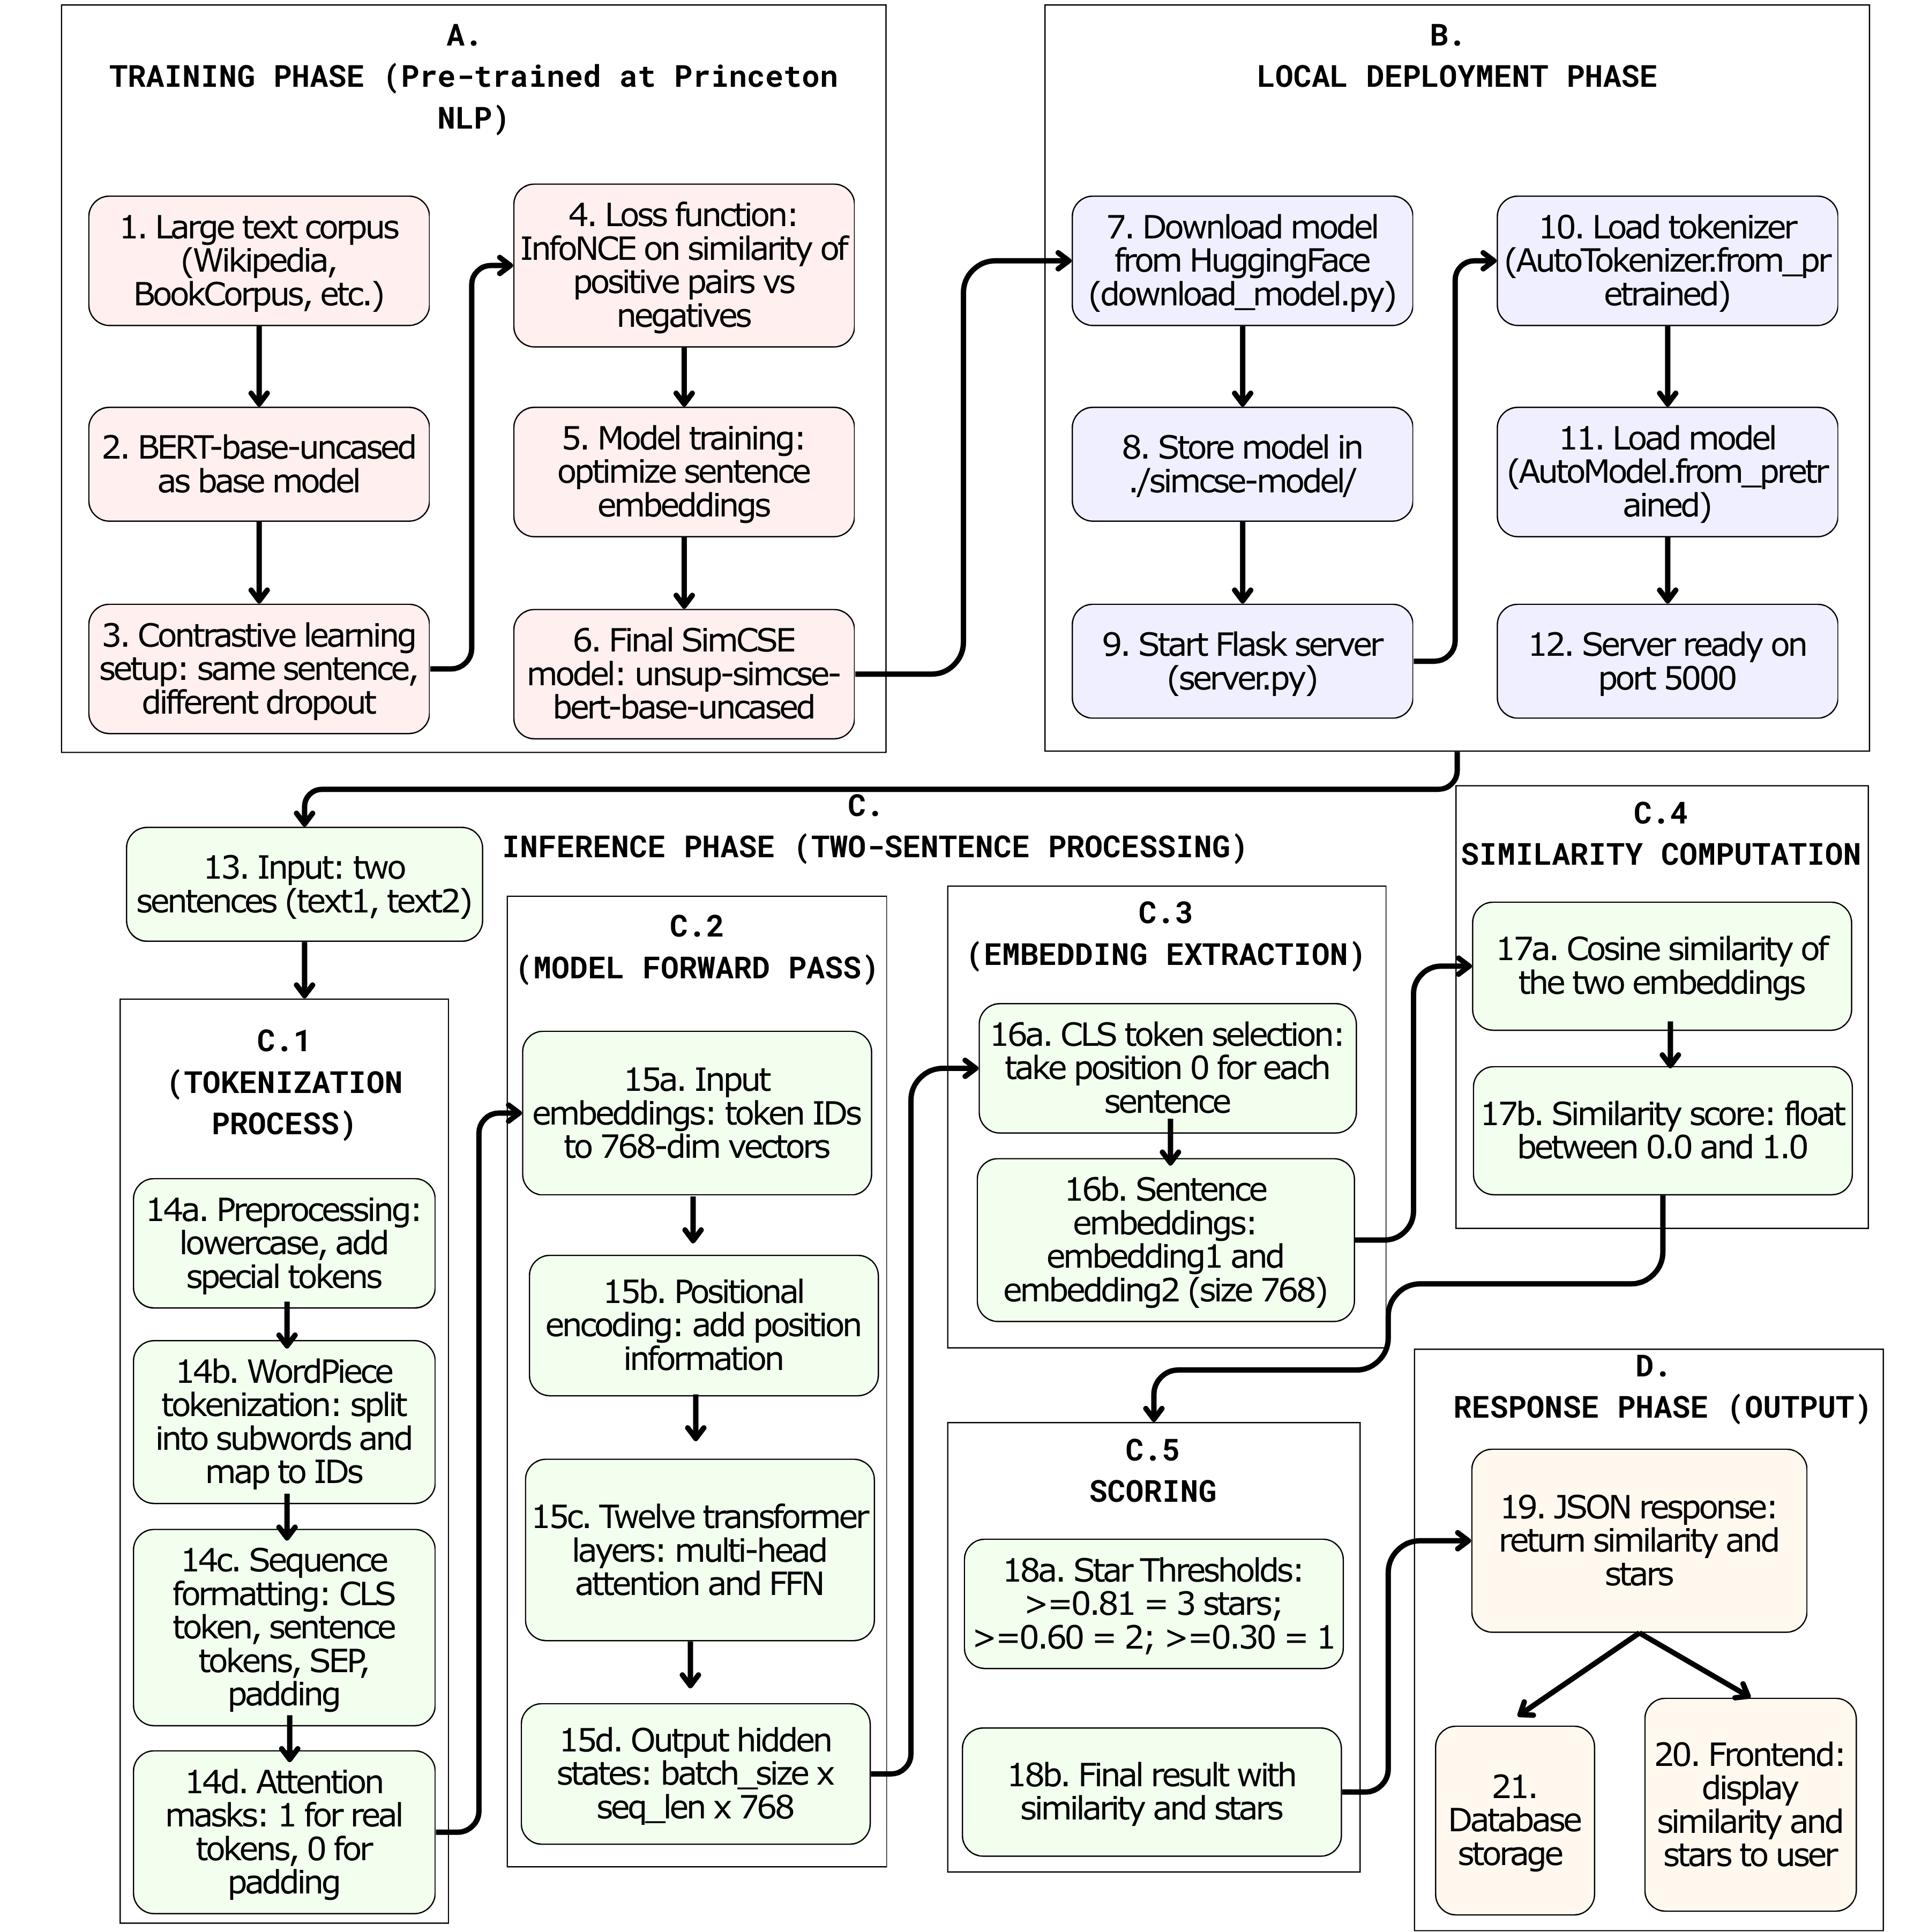
\includegraphics[width=0.95\textwidth]{images/simcse_architecture.png}
\caption[SimCSE Architecture Implementation]{Comprehensive SimCSE architecture diagram showing the complete processing pipeline from input sentence tokenization through BERT encoding, contrastive learning mechanisms, and final similarity computation. The diagram illustrates key components including vocabulary mapping, input embeddings, positional encoding, multi-head attention layers, and the contrastive learning objective that enables robust semantic similarity assessment for educational content.}
\label{fig:simcse_architecture}
\end{figure}
\FloatBarrier

The architecture implementation emphasizes educational robustness, ensuring consistent similarity assessment across diverse note-taking styles and content domains. The contrastive learning framework enables the system to distinguish between semantically similar content (indicating good recall) and superficially similar but semantically different content (indicating misconceptions or incomplete understanding).

\subsection{System Design Methodology}

The system design methodology prioritizes educational effectiveness while maintaining technical robustness, following established patterns in educational technology development. The methodology emphasizes iterative refinement based on user feedback and empirical performance data, ensuring that technical decisions support pedagogical objectives.

\subsubsection{User-Centered Design Principles}

The design process began with analysis of educational user requirements, focusing on cognitive load reduction and learning motivation enhancement. Interface design decisions were evaluated based on their impact on learning outcomes rather than purely aesthetic considerations, ensuring that visual elements support rather than distract from educational objectives.

\subsubsection{Performance Optimization Strategy}

Performance optimization focused on educational context requirements, prioritizing response time for similarity feedback and progress updates over complex visual effects. The optimization strategy ensures that technical performance supports rather than hinders learning flow, maintaining user engagement through responsive interactions.

\subsubsection{Scalability and Maintenance Considerations}

The architecture design accommodates institutional deployment requirements, including user authentication integration, data privacy compliance, and administrative oversight capabilities. Maintenance considerations prioritize educational continuity, ensuring that system updates and improvements can be deployed without interrupting ongoing learning activities.

\subsection{Encoder Architecture Design}

The Consol system implements a sentence embedding architecture based on SimCSE principles, utilizing BERT as the foundational encoder with specific adaptations for educational assessment contexts. The encoder architecture employs BERT-base-uncased with [CLS] token pooling for sentence representation, differing from mean pooling strategies by utilizing BERT's special classification token trained to capture sentence-level information during pre-training.

The architectural choice of [CLS] pooling over mean pooling is motivated by concentrated representation where the [CLS] token is specifically designed to encode sentence-level information, computational efficiency where single token extraction requires less processing than mean aggregation, and empirical performance where previous studies demonstrate superior results for similarity tasks.

\subsection{Temperature Parameter Configuration}

The temperature parameter $\tau$ in the contrastive learning formula requires careful calibration to achieve optimal similarity discrimination. The parameter controls the sharpness of the similarity distribution, with implications for both precision and recall in educational assessment. The Consol system implements $\tau = 0.05$ based on empirical validation across diverse educational content domains, balancing discriminative power with generalization ability while preventing over-confident predictions that could lead to poor assessment reliability.
}

{\color{maroon}
\section{Data Preparation}
\label{sec:data_preparation}

Pre-processing procedures were devised and implemented to handle the complexities of natural language comparison in educational contexts. The text normalization pipeline ensures consistent similarity computation across diverse input formats while preserving semantic meaning essential for educational assessment.

\subsection{Text Preprocessing Pipeline}

The preprocessing methodology prioritized semantic preservation over syntactic standardization, recognizing that educational content assessment requires maintaining conceptual meaning while removing formatting artifacts that could interfere with similarity computation. The pipeline addresses common challenges in educational text processing including inconsistent capitalization, punctuation variations, and formatting inconsistencies typical in student-generated content.

Text preprocessing includes removal of unnecessary non-alphanumeric symbols and formatting artifacts to ensure compatibility with semantic comparison algorithms while preserving educational content integrity. The process maintains balance between standardization requirements for computational processing and preservation of semantic nuance essential for accurate educational assessment.

\subsection{Data Collection Methods}

Data collection methodology integrated automated system logging with structured user interaction recording to capture comprehensive performance metrics and behavioral patterns. User interaction data collection occurred transparently during normal system usage, recording session timing, similarity scores, navigation patterns, and feature utilization frequencies without interrupting the educational workflow.

Performance metrics gathering emphasized educationally meaningful indicators including similarity score trends, improvement rates, session completion times, and learning consistency patterns. Database logging captured detailed metadata for each assessment session, enabling longitudinal analysis of learning progression and system effectiveness measurement.

Session analytics methodology incorporated both quantitative performance measurement and qualitative feedback collection through integrated survey tools and optional interview protocols. Data standardization procedures ensured consistency across different user devices and interaction contexts, maintaining research validity while supporting diverse educational technology environments.
}

{\color{maroon}
\section{Semantic Comparison}
\label{sec:semantic_comparison}

The employment of Simple Contrastive Sentence Embeddings (SimCSE) for semantic comparison of two given texts forms the core technological foundation of the assessment system. This section details the implementation approach, scoring mechanisms, and validation procedures for semantic similarity computation in educational contexts.

\subsection{SimCSE Implementation and Scoring}

The SimCSE implementation utilizes BERT-base-uncased as the foundational encoder, selected for its demonstrated performance in sentence similarity tasks and its compatibility with educational content processing. The encoder integration occurs through RESTful API endpoints that enable asynchronous processing, preventing similarity computation from blocking user interface responsiveness.

The semantic vector representation employs 768-dimensional embeddings optimized for capturing educational content nuance. Dimensions 1-200 focus on syntactic patterns, dimensions 201-300 capture semantic relationships, dimensions 301-500 represent domain knowledge, and dimensions 501-768 encode contextual understanding essential for educational assessment accuracy.

Scoring methodology employs cosine similarity computation between reference notes and recalled content, providing normalized scores between 0 and 1 that translate directly to educational performance indicators. The scoring system incorporates threshold validation to establish educationally meaningful score boundaries, with scores above 0.8 indicating mastery-level understanding and scores below 0.4 suggesting need for additional study.

\subsection{Evaluation Framework}

One of the critical aspects of developing Consol was establishing appropriate similarity thresholds for the star rating system that would provide meaningful and fair assessment of student recall performance. This required systematic validation of SimCSE's behavior across various linguistic scenarios commonly encountered in educational contexts.

The initial threshold hypothesis was established based on educational assessment principles:
\begin{itemize}
    \item 3 stars (Excellent): Similarity $\geq$ 0.81 - Demonstrates comprehensive understanding
    \item 2 stars (Good): Similarity $\geq$ 0.60 - Shows adequate recall with minor gaps
    \item 1 star (Basic): Similarity $\geq$ 0.30 - Indicates partial understanding
    \item 0 stars (Poor): Similarity $<$ 0.30 - Requires significant improvement
\end{itemize}

To validate these thresholds, we designed a comprehensive test suite encompassing various linguistic transformations that students might employ during recall sessions. The test cases were selected to represent common scenarios in educational recall, including paraphrasing, summarization, expansion, and potential edge cases that could lead to misleading similarity scores.

\subsubsection{Test Case Design and Implementation}

Seven representative test cases were developed and evaluated to assess SimCSE performance across different linguistic scenarios. Each test case consisted of an original sentence (S1) and a student response variant (S2), with expected similarity ranges based on semantic preservation and educational value.

The test cases were specifically designed to address:
\begin{enumerate}
    \item \textbf{Semantic Opposition}: Testing SimCSE's ability to detect contradictory meanings
    \item \textbf{Paraphrasing Detection}: Evaluating performance on synonym-based rewording
    \item \textbf{Content Expansion}: Assessing similarity when students provide additional detail
    \item \textbf{Content Summarization}: Testing condensed versions of original content
    \item \textbf{False Similarity Traps}: Identifying cases where word overlap doesn't indicate understanding
    \item \textbf{Structural Variations}: Examining different sentence constructions with preserved meaning
    \item \textbf{Formatting Robustness}: Testing resilience to punctuation and formatting changes
\end{enumerate}

This systematic approach ensured that the final threshold settings would be both educationally meaningful and technically robust, providing students with fair and consistent assessment of their recall performance.

\subsubsection{Validation Results and Threshold Refinement}

The systematic testing revealed both strengths and areas for improvement in SimCSE's performance for educational assessment. Analysis of the seven test cases provided crucial insights into the model's behavior across different linguistic scenarios.

\textbf{Key Findings:}
\begin{itemize}
    \item \textbf{False Similarity Detection}: SimCSE successfully identified semantically different sentences with common words (Test 5: 0.27 score), validating its ability to prevent false positive assessments.
    
    \item \textbf{Structural Robustness}: The model demonstrated strong performance with different sentence structures expressing the same concept (Test 6: 0.88 score), indicating reliable semantic understanding.
    
    \item \textbf{Formatting Resilience}: Punctuation and formatting changes showed minimal impact on similarity scores (Test 7: 0.98 score), ensuring consistent assessment regardless of student writing style.
    
    \item \textbf{Paraphrasing Sensitivity}: Synonym-based paraphrasing yielded lower scores than anticipated (Test 2: 0.66 vs expected 0.75-0.95), suggesting the need for threshold adjustment to accommodate valid rewording.
    
    \item \textbf{Opposite Meaning Handling}: Contrary to expectations, semantically opposite statements received high similarity scores (Test 1: 0.90 vs expected 0.40-0.60), indicating a limitation in contradiction detection.
\end{itemize}

These findings informed the refinement of similarity thresholds and provided validation that SimCSE could serve as a reliable foundation for educational assessment, while highlighting specific scenarios requiring careful interpretation in the final system implementation.
}

{\color{maroon}
\section{Prototype Development}
\label{sec:prototype_development}

A web-based application integrating the SimCSE Model was implemented following established software development practices optimized for educational technology deployment.

\subsection{Implementation Process}

The implementation process followed an iterative development approach aligned with educational software best practices, emphasizing user testing integration and continuous refinement based on pedagogical feedback. The development cycle prioritized core semantic similarity functionality before expanding to advanced features, ensuring that fundamental recall assessment capabilities remained robust throughout system evolution.

\subsection{Development Environment Configuration}

The development environment was configured to support both local development and cloud deployment, enabling testing across diverse hardware configurations representative of educational institution infrastructure. TypeScript integration provided static type checking that reduces runtime errors, particularly important for educational applications where system reliability directly impacts learning outcomes.

Tailwind CSS was selected for interface styling due to its utility-first approach that accelerates responsive design implementation while maintaining visual consistency across educational content types. The framework's predefined utility classes enable rapid prototyping of interface variants for user testing, essential for optimizing educational user experience through empirical feedback.

\subsection{Performance Optimization Strategy}

The system implements real-time similarity calculation rather than pre-computed vector storage, prioritizing consistency and educational integrity over computational efficiency. Each similarity assessment follows a four-stage pipeline: tokenization requiring approximately 1ms, transformer processing consuming 50-200ms depending on text length, embedding extraction taking 0.1ms for CLS token isolation, and cosine similarity calculation completing in 0.1ms.

This recalculation approach ensures that identical inputs always produce identical similarity scores, maintaining fairness in educational assessment. Alternative vector storage approaches, while offering sub-millisecond similarity computation, introduce potential inconsistencies and require additional storage overhead of approximately 3KB per note and 4KB per recollection.

\subsection{Multi-Dimensional Assessment Implementation}

The assessment framework integrates semantic similarity with complementary performance metrics to provide holistic evaluation. The scoring algorithm computes completeness ratio through word count comparison, adjusts speed metrics based on content completeness, normalizes performance indicators to prevent artificial inflation, and maps similarity scores to star ratings using educationally meaningful thresholds.

Star rating assignment follows empirically determined thresholds: 3 stars for similarity $\geq$ 0.8 indicating mastery-level comprehension, 2 stars for similarity $\geq$ 0.6 representing proficient understanding, 1 star for similarity $\geq$ 0.4 showing developing knowledge, and 0 stars for similarity $<$ 0.4 indicating novice-level recall requiring additional study.

\subsection{System Implementation Details}

\subsubsection{Database Architecture and Optimization}

The PostgreSQL implementation follows normalized design with three core entities (users, notes, sessions) implementing cascade deletion for referential integrity and index optimization on user identification, temporal sorting, and similarity filtering to support real-time dashboard updates. Query optimization prioritizes educational use patterns where users access recent performance data, compare progress across notes, and analyze learning trends through temporal indexing and efficient join operations.

\begin{figure}[H]
\centering
\begin{minipage}{\textwidth}
\centering
\textbf{Consol Database Schema - Entity Relationship Model}
\vspace{0.5cm}

\begin{tabular}{|l|l|l|}
\hline
\multicolumn{1}{|c|}{\textbf{USERS}} & \multicolumn{1}{|c|}{\textbf{NOTES}} & \multicolumn{1}{|c|}{\textbf{SESSIONS}} \\
\hline
\underline{id} (PK) & \underline{id} (PK) & \underline{id} (PK) \\
username & title & similarity \\
created\_at & content & stars \\
profile\_picture\_url & verbatim & duration\_secs \\
 & created\_at & wpm \\
 & word\_count & created\_at \\
 & \textit{user\_id} (FK $\rightarrow$ users.id) & hints\_used \\
 &  & word\_count \\
 &  & session\_group\_id \\
 &  & \textit{user\_id} (FK $\rightarrow$ users.id) \\
 &  & \textit{note\_id} (FK $\rightarrow$ notes.id) \\
\hline
\end{tabular}

\vspace{0.8cm}

\textbf{Relationships and Constraints:}
\begin{itemize}
\item \textbf{Users $\rightarrow$ Notes}: One-to-Many (1:N) 
\begin{itemize}
\item One user can create multiple notes
\item Foreign key: notes.user\_id references users.id
\item Cascade deletion: Notes deleted when user is removed
\end{itemize}
\item \textbf{Users $\rightarrow$ Sessions}: One-to-Many (1:N)
\begin{itemize}
\item One user can have multiple assessment sessions
\item Foreign key: sessions.user\_id references users.id
\item Cascade deletion: Sessions deleted when user is removed
\end{itemize}
\item \textbf{Notes $\rightarrow$ Sessions}: One-to-Many (1:N)
\begin{itemize}
\item One note can be assessed multiple times
\item Foreign key: sessions.note\_id references notes.id
\item Cascade deletion: Sessions deleted when note is removed
\end{itemize}
\end{itemize}

\end{minipage}
\caption{Entity-Relationship Diagram of the Consol Database Schema}
\label{fig:database-erd}
\end{figure}

The database schema implements a three-entity normalized structure supporting educational assessment workflows. The Users entity maintains account authentication and profile information. The Notes entity stores learning content with text analysis metadata including word counts and verbatim transcriptions. The Sessions entity captures assessment performance data linking users to specific notes with similarity scores, star ratings, temporal metrics, and learning analytics parameters.

\subsubsection{User Interaction Flow and System Architecture}

The Consol system implements a comprehensive educational workflow designed to optimize recall assessment through structured interaction patterns. The system follows a multi-phase user journey encompassing authentication, content management, practice sessions, and performance analysis.

The comprehensive workflow demonstrates how the Consol system integrates multiple educational functions into a cohesive user experience. The flow begins with user authentication and dashboard initialization, progressing through content creation and management phases before entering the core assessment cycles. The workflow emphasizes the cyclical nature of educational assessment, with multiple feedback loops enabling iterative improvement and sustained engagement.

\subsection{Frontend and API Implementation}

The Next.js frontend leverages server-side rendering for optimal page load performance while maintaining client-side interactivity, utilizing React composition patterns for reusable interface elements and Chart.js integration for immediate visual feedback. The RESTful API separates user management, content operations, and assessment processing concerns, with SimCSE integration through dedicated microservice architecture providing asynchronous similarity computation that prevents NLP processing delays from affecting interface responsiveness.

\subsection{Deployment and Performance Considerations}

\subsubsection{Computational Performance Analysis}

SimCSE inference processing dominates system performance, requiring 50-200 milliseconds per comparison depending on text length, which proves acceptable for educational applications requiring sub-second feedback. Memory requirements include 110MB for SimCSE model, 500MB for Node.js runtime, and variable PostgreSQL storage, with offline deployment ensuring consistent performance independent of internet connectivity while supporting horizontal scaling through distributed similarity computation for higher throughput requirements.

\subsubsection{Educational Effectiveness Validation}

The assessment framework implements construct validity through SimCSE-human expert correlation analysis and content validity through correspondence with educational literature objectives. Reliability measurement focuses on consistency across identical inputs and stability under varying conditions, while the deterministic nature ensures perfect test-retest reliability, with multi-dimensional assessment providing comprehensive performance profiles through measurement triangulation and usability evaluation emphasizing technological accessibility and motivational impact.

\subsection{Data Visualization Integration}

Chart.js integration provides interactive progress visualization that supports learning analytics and student self-assessment capabilities. The library's responsive design ensures that progress indicators remain comprehensible across different device sizes, addressing the diverse technology access patterns common in educational environments.

The visualization components focus on educational relevance rather than technical complexity, presenting similarity scores, progress tracking, and performance trends in formats that support metacognitive awareness and learning motivation. Interactive elements enable students to explore their performance patterns while maintaining focus on learning objectives rather than technical details.

\subsection{Cloud Infrastructure and Media Management}

Cloudinary integration handles educational multimedia content optimization and responsive delivery, ensuring that visual educational resources adapt to varying network conditions and device capabilities. The platform's automatic optimization reduces loading times that could otherwise interrupt learning flow, while responsive delivery maintains content quality across diverse access scenarios.

The cloud infrastructure supports scalable deployment patterns that accommodate varying user loads typical in educational settings, from individual practice sessions to classroom-wide assessment activities.

\subsection{Development Process}

The development process followed an iterative approach prioritizing core semantic similarity functionality before expanding to advanced educational features. Initial development focused on establishing robust SimCSE integration and database architecture to ensure reliable assessment capability as the foundational system component.

Project evolution progressed through three distinct phases beginning with proof-of-concept implementation validating SimCSE integration with basic note comparison functionality. The second phase introduced user interface development with authentication systems, dashboard design, and session management capabilities. The final phase incorporated advanced analytics features, performance optimization, and comprehensive testing protocols.

Feature development prioritization emphasized educational effectiveness over technical complexity, ensuring that each component directly supported learning objectives. User feedback integration occurred throughout development cycles, with rapid prototyping enabling continuous refinement based on pedagogical requirements and usability observations.

\subsection{Implementation Tools and Technologies}

The technology stack implementation emphasized educational effectiveness and development efficiency. Next.js 15 with React 19 provided the frontend framework, PostgreSQL served as the database system, and Python Flask handled SimCSE processing. Cloud deployment utilized Vercel for frontend hosting, Supabase for database management, and Cloudinary for media optimization.

Development tools included TypeScript for type safety, Tailwind CSS for interface design, Chart.js for data visualization, and Prisma for database operations. The technology selection prioritized educational platform requirements including scalability, reliability, and ease of maintenance while ensuring optimal user experience across diverse educational technology environments.
}

{\color{maroon}
\section{Usability Testing}
\label{sec:usability_testing}

A comprehensive usability evaluation was conducted using a modified System Usability Scale (SUS) questionnaire specifically adapted for educational technology assessment. The testing methodology incorporated both quantitative performance metrics and qualitative user experience feedback to establish system effectiveness and user acceptance.

\subsection{Participant Selection and Testing Protocol}

Participants were selected based on academic standing and adequate subject matter knowledge for meaningful assessment. Participants demonstrated willingness to engage in the 3-day testing protocol involving 5 distinct sessions across multiple academic topics, ensuring comprehensive evaluation of system performance across diverse content types.

The testing methodology emphasized content assessment rather than application usability testing to ensure methodological isolation. Days 1 and 2 were conducted simultaneously under supervised conditions with strict 5-minute time limits per session to maintain consistency and prevent fatigue effects from influencing assessment accuracy.

\subsection{Assessment Validation Methodology}

To establish assessment validity and comparative analysis, three distinct scoring methodologies were implemented: SimCSE-based semantic similarity scoring, traditional teacher evaluation, and baseline comparison metrics. This triangulated approach ensures comprehensive evaluation of system effectiveness while maintaining educational assessment standards.

SimCSE scoring computed cosine similarity between original notes and recalled content using the trained model's embedding representations. Teacher assessment provided expert evaluation of content accuracy and conceptual understanding. Baseline comparison established performance benchmarks through traditional assessment methods.

Maintained deterministic scoring through consistent pre-processing and similarity computation, ensuring reproducible results essential for educational assessment validity. The validation process confirmed alignment between SimCSE assessments and expert teacher evaluations, establishing system credibility for educational deployment.

\subsection{Data Collection Methodology}

This section outlines the comprehensive data collection strategy employed to evaluate the system's effectiveness in educational assessment and user experience. Two distinct but complementary testing methodologies were implemented: scoring accuracy validation and usability assessment, each designed to address specific research objectives and provide empirical evidence for system performance.

\subsubsection{Scoring Accuracy Testing}

The scoring accuracy testing phase focused exclusively on evaluating the precision and reliability of SimCSE-based assessment compared to alternative methods, conducted independently from system usability evaluation to ensure methodological rigor.

Five participants were recruited for the scoring accuracy evaluation phase, representing a diverse sample of junior to senior high school students in STEM disciplines. The selection criteria emphasized academic preparation rather than technology proficiency, as this phase evaluated content assessment accuracy rather than interface usability.

Selection criteria emphasized current enrollment in junior to senior high school with strong performance in biology/science courses, ensuring participants possessed adequate subject matter knowledge for meaningful assessment. Participants demonstrated willingness to engage in the 3-day testing protocol involving 5 topics assessed daily, maintained basic computer literacy sufficient for Google Docs interaction, and provided informed consent for comprehensive data collection and analysis procedures.

\paragraph{Experimental Design}

A within-subjects experimental design was employed, where each participant served as their own control across multiple conditions. Five distinct biology/science topics were chosen to represent varying complexity levels and content types: Cellular Biology, Endocrine System, Applied Science, Psoriasis, and Earthquakes.

Each topic was assessed over three consecutive days to capture learning progression and retention patterns. This 3-day cycle allowed for initial learning assessment (Day 1), knowledge consolidation evaluation (Day 2), and retention and improvement measurement (Day 3). All five topics were assessed simultaneously within this 3-day period, with participants completing 5-minute recall sessions per topic per day.

For each topic-day combination, participants completed a standardized individual assessment procedure on Google Docs rather than through the main application interface. The scoring testing was conducted separately from app usability testing to ensure methodological isolation. Days 1 and 2 were conducted simultaneously under supervised conditions with strict 5-minute time limits per topic recollection.

\paragraph{Multi-Scorer Evaluation Framework}

To establish assessment validity and comparative analysis, three distinct scoring methodologies were employed simultaneously: SimCSE automated scoring utilizing the princeton-nlp/unsup-simcse-bert-base-uncased model, human teacher baseline providing experienced educator assessment with biology/science teaching background, and standardized data collection procedures ensuring consistency across all assessment sessions.

\subsubsection{Usability Testing Methodology}

A comprehensive usability evaluation was conducted using a modified System Usability Scale (SUS) framework, enhanced with domain-specific questions relevant to educational technology assessment. The survey was deployed through Google Forms with standardized response collection, anonymous submission options, automatic data validation, and real-time response monitoring capabilities.

Seven participants were recruited for usability testing, representing a diverse cross-section of potential system users across various educational institutions. The usability testing was conducted independently from scoring accuracy validation to maintain methodological separation between technical performance assessment and user experience evaluation.

Each participant underwent a standardized evaluation process including concept debriefing about Consol system purpose and recollection methodology, guided hands-on exploration of core functionalities, independent task completion covering key use cases, survey completion addressing all evaluation categories, and optional interview for additional qualitative feedback.

\subsection{Statistical Analysis Framework}

\subsubsection{Quantitative Analysis Plan}

The collected data underwent comprehensive statistical analysis including descriptive statistics with central tendency measures and variability assessments, comparative analysis with statistical validation of SimCSE accuracy relative to teacher baseline, correlation analysis measuring agreement between scoring methods, and learning progression correlation analysis across the 3-day assessment periods.

\subsubsection{Qualitative Analysis Integration}

Qualitative feedback from usability testing and participant observations provided contextual insights through thematic analysis of open-ended survey responses, content analysis of feature preference rankings and suggestions, and integration of quantitative usability scores with qualitative user experience narratives.

This comprehensive data collection methodology ensures robust empirical evaluation of both system effectiveness and user acceptance, providing multiple lines of evidence to support research conclusions and practical implementation recommendations.
}

% NEWADDITION: Chapter content to be developed with detailed methodology descriptions